
\renewcommand{\thechapter}{T}
\setcounter{section}{0}
\chapter{Таблице}


\section{Конволуција континуалних сигнала}

Конволуција континуалних сигнала $x(t)$ и $y(t)$ у општем случају дефинише се као 
$x(t) \ast y(t) = \int_{\uptau = -\infty}^{\infty} x(\uptau) y(t - \uptau) \, \de \uptau$.

\begin{center}
    \noindent
    \begin{tabular}{|c|c|c|c|} \hline
        рбр. & $x(t)$ & $y(t)$ & $x\ast y (t)$  
        \\ \hline \hline
        \rule{0pt}{4ex}  
        % (1)
        \redTablice &
        ${\rm e}^{\uplambda t}$\,{\rm u}(t) & 
        ${\rm e}^{\uplambda t}$\,{\rm u}(t) & 
        $\dfrac{1}{2} t {\rm e}^{\uplambda t} \,{\rm u}(t)$ 
        \\ \rule{0pt}{4ex}  
        % (2)
        \redTablice &
        $t^N\,{\rm u}(t)$ &
        ${\rm e}^{\uplambda t}\,{\rm u}(t)$ &
        $\displaystyle
        \left( \dfrac{N! {\rm e}^{\uplambda t}}{\uplambda^{N+1}} 
        - 
        \sum_{k=0}^N \dfrac{N! t^{N-k}}{
        \uplambda^{k+1}(N-k)!} \right) \, {\rm u}(t)
        $ \\  \rule{0pt}{4ex}   
        \redTablice \label{T:ctc:rect}& 
        $\rect(t)$ & $\rect(t)$ & $\tri(t)$ \\ \rule{0pt}{4ex}   
        % (3)
        \redTablice &
        $t^M\,{\rm u}(t)$ & $t^N\,{\rm u}(t)$ & 
        $
        \dfrac{M! N!}{(N+M+1)!} t^{N + M + 1} \, {\rm u}(t)
        $ \\ \rule{0pt}{4ex}  
        % (4)
        \redTablice &
        $t {\rm e}^{\uplambda_1 t} \,{\rm u}(t)$ & 
        ${\rm e}^{\uplambda_2 t} \,{\rm u}(t)$ &
        $
        \dfrac{ {\rm e}^{\uplambda_2 t} - {\rm e}^{\uplambda_1 t} 
        + ( \uplambda_1 - \uplambda_2 )t {\rm e}^{\uplambda_1 t} }
        {( \uplambda_1 - \uplambda_2 )^2} \, {\rm u}(t)
        $ \\ \rule{0pt}{4ex} 
        % (5)
        \redTablice &
        $t^M {\rm e}^{\uplambda t} \,{\rm u}(t)$ & $t^N
        {\rm e}^{\uplambda t}\,{\rm u}(t)$ & 
        $ 
        \dfrac{M! N!}{(N+M+1)!} t^{N + M + 1} {\rm e}^{\uplambda t}\, {\rm u}(t)
        $ \\ \rule{0pt}{4ex}  
        % (6)
        \redTablice &
        $ {\rm e}^{-\upsigma t} \cos({\upomega t + \uptheta})\,{\rm u}(t) $ &
        $ {\rm e}^{\uplambda t}\,{\rm u}(t) $ &
        $
        \dfrac{\cos(\uppsi) {\rm e}^{\uplambda t} -
        {\rm e}^{-\upsigma t} \cos(\upomega t + \uppsi) }
        {\sqrt{ \upomega^2 + (\upsigma + \uplambda)^2 }}
        \, {\rm u}(t) $ \\
        & & & где су $\upphi = {\rm arg}( (\upsigma + \uplambda) + 
        {\rm j}\upomega ) $, и2
        \\
        & & & $\uppsi = \uptheta-\upphi$ \\
        \hline
    \end{tabular}
\end{center}


\section{Конволуција дискретних сигнала}

Конволуција континуалних сигнала $x[n]$ и $y[n]$ у општем случају дефинише се као 
$x[n] \ast y[n] = \sum_{m = -\infty}^{\infty} x[m] y[n-m]$.

\begin{center}   
    {\tabulinesep=0.2mm
    \begin{tabu}{|c|c|c|c|} \hline
        рбр. & $x[n]$ & $y[n]$ & $x\ast y [n]$  
        \\ \hline \hline
        %\rule{0pt}{4ex}  
        % (1)
        \redTablice &
        $\uplambda^n\, {\rm u}[n]$
        &	
        $\uplambda^n\, {\rm u}[n]$
        &
        $(1+n)\uplambda^n \, {\rm u}[n]$
        \\ %\hline 
        \rule{0pt}{4.5ex} 
        % (2)
        \redTablice &
        $n\, {\rm u}[n]$
        &
        $\uplambda^n\, {\rm u}[n]$
        &
        $
        \dfrac{\uplambda^{n+1} - 
        \uplambda(1+n)+n}{(\uplambda - 1)^2}
        \, {\rm u}[n]
        $
        \rule{0pt}{4.5ex}
        \\ %\hline 
        \rule{0pt}{4.5ex} 
        % (3)
        \redTablice &
        $n \lambda_1^n\, {\rm u}[n]$ 
        &
        $\lambda_2^n\, {\rm u}[n]$ 
        &
        $
        - \frac{\lambda_{1} \left(\lambda_{1}^{n} \lambda_{2} n + \lambda_{1}^{n} \lambda_{2} - \lambda_{1}^{n + 1} n - \lambda_{2}^{n + 1}\right)}{\left(\lambda_{1} - \lambda_{2}\right)^{2}}
        \, {\rm u}[n]
        $
        \\ %\hline 
        \rule{0pt}{4.5ex} 
        % (4)
        \redTablice &
        $n \lambda^n\, {\rm u}[n]$ 
        &
        $\lambda^n\, {\rm u}[n]$ 
        &
        $
        \frac{\lambda^{n} n \left(n + 1\right)}{2}
        \, {\rm u}[n]
        $
        \\ \hline
        %\rule{0pt}{4.5ex}
    \end{tabu} }
\end{center}

\section{Неки формални развоји} \label{T:frs}

За $|a| < 1$ важе развоји на основном 
периоду $T_{\rm F} = T_ 0 = 
\dfrac{2\uppi}{\upomega}$

\begin{center}
    \begin{tabular}{|c|c|}\hline
    рбр. & развој \\ \hline \hline
    \redTablice &
    $
    \dfrac{a\sin(\upomega t)}{
    1 - 2a \cos(\upomega t) + a^2} = 
    \sum_{k = 0}^{\infty} a^k \sin(k\upomega t), \;
    $ \\
    \redTablice &
    $
    \dfrac{1 - a^2}{
    1 - 2a \cos(\upomega t) + a^2} = 
    1 + 2
    \sum_{k = 1}^{\infty} a^k \cos(k\upomega t),
    $ \\
    \redTablice &
    $
    \dfrac{1 - a \cos{\upomega t}}{
    1 - 2a \cos(\upomega t) + a^2} = 
    \sum_{k = 0}^{\infty} a^k \cos(k\upomega t),
    $ \\ \hline
    \end{tabular}
\end{center}

\section{Неки таблични интеграли}

\begin{center}
    \begin{enumerate}
    \item[\redTablice] $\int \mathrm{e}^{at} \, P_n(t) \, dt = C + \dfrac{\mathrm{e}^{at}}{a} \, \displaystyle \sum_{k=0}^{n} \dfrac{(-1)^k}{a^k} \, \dfrac{{\rm d}^k P_n(t)}{
    {\rm d}t^k}$, где је $P_n$ полином $n$-тог реда 
    
    \item[\redTablice] $\int \mathrm{e}^{at} \, \cos(bt) \, {\rm d}t = C + \dfrac{\mathrm{e}^{at} \, (a \, \cos(bt) + b \, \sin(bt))}{a^2 + b^2}$
    \item[\redTablice\label{T:int:esin}] $\int \mathrm{e}^{at} \, \sin(bt) \, dt = C + \dfrac{\mathrm{e}^{at} \, (-b \, \cos(bt) + a \, \sin(bt))}{a^2 + b^2}$ 
    \item[\redTablice] $\int \mathrm{e}^{at} \, b^t \, dt = C + \dfrac{b^t \, \mathrm{e}^{at}}{a + \ln(b)}$, $b>0$, $a \neq -\ln(n)$
    \end{enumerate}
\end{center}

\clearpage
\section{Фуријеови редови континуалних сигнала} 

\begin{center}
    \newcommand*{\figscale}{0.75}
    { \tabulinesep=0.2mm
    \begin{tabu}{|c|c|c|c|}
    \hline
    рбр. & Основни период $x(t)$ & $X[k] = \FS{x(t)}$ & Период развоја \\ \hline \hline
    \redTablice \label{t:ctfs:comb} &
    $\updelta(t)$ & $\operatorname{comb}_m[k]$ & $T_{\rm F} = m \, T_0$ \\
    & 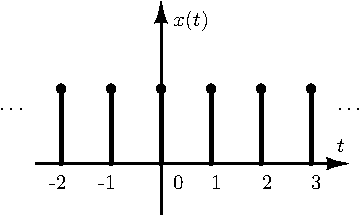
\includegraphics[scale=\figscale]{fig/t_3_1.pdf} & 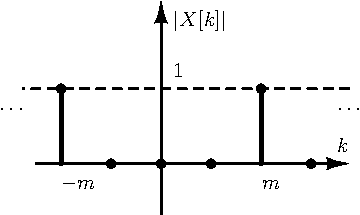
\includegraphics[scale=\figscale]{fig/t_3_2.pdf} & \\
    \hline
    \redTablice \label{T:ctfs:rect}&
    $\operatorname{rect}\left(\frac{t}{w}\right)$ & $\frac{w}{T_0} \, \operatorname{sinc}\left(\frac{k \, w}{T_0}\right)$ & $T_{\rm F} = T_0$\\
    & 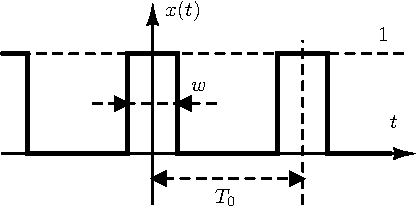
\includegraphics[scale=\figscale]{fig/t_3_3.pdf} &&\\
    \hline
    \redTablice &
    $\operatorname{tri}\left(\frac{t}{w}\right)$ & $\frac{w}{T_0} \, \operatorname{sinc}^2\left(\frac{k\,w}{T_0}\right)$ & $T_{\rm F} = T_0$\\
    & 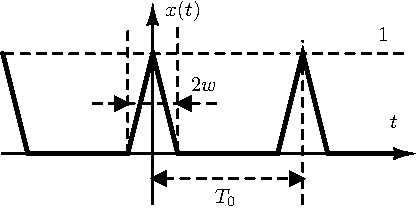
\includegraphics[scale=\figscale]{fig/t_3_4.pdf} &&\\
    \hline
    \redTablice &
    $\operatorname{sinc}\left(\frac{t}{w}\right)$ & $\frac{w}{T_0} \, \operatorname{rect}\left(\frac{k\,w}{T_0}\right)$ & $T_{\rm F} = T_0$ \\
    \hline
    \end{tabu} }
\end{center}

\section{Фуријеове трансформације континуалних сигнала}

\begin{center}
    {\tabulinesep=1.2mm
    \begin{tabu}{|c|c|c|} 
    \hline
    рбр & $x(t)$ & $X(\jj \upomega) = \FT{x(t)}$ \\
    \hline \hline
    \redTablice & $1$ & $2\uppi \, \updelta(\upomega)$ \\
    \hline
    \redTablice & $\updelta(t)$ & $1$ \\
    \hline
    \redTablice \label{T:ctft:uu} & $\mathrm{u}(t)$ & $\dfrac{1}{\jj\upomega} + \uppi \, \updelta(\upomega)$ \\
    \hline 
    \redTablice & $\mathrm{e}^{\jj\upomega_0 t}$ & $2\uppi \, \updelta(\upomega-\upomega_0)$ \\
    \hline 
    \redTablice & $\mathrm{rect}(t)$ & $\mathrm{sinc}\left(\frac{\upomega}{2\uppi}\right)$ \\
    \hline 
    \redTablice \label{T:ctft:sinc} & $\mathrm{sinc}(t)$ & $\mathrm{rect}\left(\frac{\upomega}{2\uppi}\right)$ \\
    \hline 
    \redTablice & $\mathrm{comb}(t)$ & $\mathrm{comb}\left(\frac{\upomega}{2\uppi}\right)$ \\
    \hline 
    \redTablice \label{T:ctft:cos} & $\cos(\upomega_0 t)$ & $\uppi \, \bigl(\updelta(\upomega + \upomega_0) + \updelta(\upomega - \upomega_0)\bigr)$ \\
    \hline
    \redTablice \label{T:ctft:sin} & $\sin(\upomega_0 t)$ & $\jj\uppi \, \bigl(\updelta(\upomega + \upomega_0) - \updelta(\upomega - \upomega_0)\bigr)$ \\
    \hline 
    \redTablice & $\mathrm{sinc}^2(t)$ & $\mathrm{tri}\left(\frac{\upomega}{2\uppi}\right)$ \\
    \hline
    \redTablice & $\mathrm{tri}(t)$ & $\mathrm{sinc}^2\left(\frac{\upomega}{2\uppi}\right)$ \\
    \hline
    \redTablice & $\mathrm{e}^{-at} \, \mathrm{u}(t), \quad \Re a > 0$ & $\dfrac{1}{a + \jj\upomega}$ \\
    \hline
    \redTablice & $\mathrm{e}^{-\uppi t^2}$ & $\mathrm{e}^{-\frac{\upomega^2}{4\uppi}}$ \\
    \hline
    \redTablice & $\dfrac{t^{n-1}}{(n-1)!} \, \mathrm{e}^{-at} \, \mathrm{u}(t), \quad \Re a > 0$ &  $\dfrac{1}{(a+\jj\upomega)^n}$ \\
    \hline
    \redTablice & $\mathrm{e}^{-at} \, \cos(\upomega_0 t) \, \mathrm{u}(t), \quad \Re a > 0$ & $\dfrac{a+\jj\upomega}{(a+\jj\upomega)^2 + \upomega^2_0}$ \\
    \hline
    \redTablice & $\mathrm{e}^{-at} \, \sin(\upomega_0 t) \, \mathrm{u}(t), \quad \Re a > 0$ & $\dfrac{\upomega_0}{(a+\jj\upomega)^2 + \upomega^2_0}$ \\ \hline
    \end{tabu}
    }
\end{center}

\section{Унилатерална Лапласова трансформација}

\begin{center}
    {\tabulinesep=1.2mm
    \begin{tabu}{|c|c|c|} 
    \hline
    рбр & $x(t)$ & $X(s) = \mathcal{L} \{x(t)\}$ \\
    \hline \hline
    \redTablice & $\updelta(t)$ & $1$ \\
    \hline
    \redTablice \label{T:LT:u}& $\mathrm{u}(t)$ & $\dfrac{1}{s}$ \\
    \hline 
    \redTablice & $\dfrac{1}{\sqrt{\uppi t}}\,\mathrm{u}(t)$ & $\dfrac{1}{\sqrt{s}}$ \\
    \hline 
    \redTablice & $2 \, \sqrt{\dfrac{t}{\uppi}}\,\mathrm{u}(t)$ & $s^{-\frac{3}{2}}$ \\
    \hline 
    \redTablice & $\dfrac{t^n}{n!}\,\mathrm{u}(t), \quad n\in\mathbb N$ & $\dfrac{1}{s^{n+1}}$ \\
    \hline 
    \redTablice & $\mathrm{e}^{-at}\,\mathrm{u}(t)$ & $\dfrac{1}{s+a}$ \\
    \hline 
    \redTablice & $\dfrac{t^{n-1} \, \mathrm{e}^{-at}}{(n-1)!}\,\mathrm{u}(t), \quad n\in\mathbb N$ & $\dfrac{1}{(s+a)^n}$ \\
    \hline
    \redTablice & $\cos(\upomega t)\,\mathrm{u}(t)$ & $\dfrac{s}{s^2 + \upomega^2}$ \\
    \hline 
    \redTablice \label{T:LT:sin}& $\sin(\upomega t)\,\mathrm{u}(t)$ & $\dfrac{\upomega}{s^2 + \upomega^2}$ \\
    \hline
    \redTablice & $\cosh(\upomega t)\,\mathrm{u}(t)$ & $\dfrac{s}{s^2 - \upomega^2}$ \\
    \hline
    \redTablice & $\sinh(\upomega t)\,\mathrm{u}(t)$ & $\dfrac{\upomega}{s^2 - \upomega^2}$ \\
    \hline
    \redTablice & $\dfrac{t}{2\upomega} \, \sin(\upomega t)\,\mathrm{u}(t)$ & $\dfrac{s}{(s^2 + \upomega^2)^2} $ \\
    \hline
    \redTablice & $\dfrac{\sin(\upomega t) - \upomega t \, \cos(\upomega t)}{2 \upomega}\,\mathrm{u}(t)$ & $\dfrac{\upomega^2}{(s^2 + \upomega^2)^2}$ \\
    \hline
    \redTablice\label{T:LT:exp_sin} &
    ${\rm e}^{-at} \sin(\upomega t)\,\mathrm{u}(t)$
    &
    $
    \dfrac{\upomega}{(s+a)^2 + \upomega^2}
    $ \\ \hline
    \redTablice\label{T:LT:exp_cos} &
    $ 
    {\rm e}^{-at} \cos(\upomega t)\,\mathrm{u}(t)
    $
    &
    $
    \dfrac{s + a}{(s+a)^2 + \upomega^2}
    $ \\ \hline
    \end{tabu}
    }
\end{center}

\section{Фуријеова трансформација дискретног сигнала}

\begin{center}
    {\tabulinesep=1.2mm
    \begin{tabu}{|c|c|c|} 
    \hline
    рбр & $x[n]$ & $X(\jj\Omega) = \FT{x[n]}$ \\
    \hline \hline
    %(1) 
    \redTablice &
    $\updelta[n]$ & $1$ \\
    \hline
    %(2)
    \redTablice &
    $\updelta[n-N]$ & $\ee^{-\jj\Omega N}$ \\
    \hline
    %(4)
    \redTablice &
    $
    \sum\limits_{p=-\infty}^{+\infty} \updelta[n-p\, N]$ & $\dfrac{2\uppi}{N} \, 
    \operatorname{rep}_{\frac{2\uppi}{N}} 
    \updelta\left(\Omega\right)$ \\
    \hline
    %(5)
    \redTablice &
    $1$ & $2\uppi 
    \operatorname{rep}_{2\uppi}
    \updelta(\Omega)$ \\
    \hline
    % (6)
    \redTablice &
    $\operatorname{sgn}[n]$ & $\dfrac{2}{1 - \ee^{-\jj\Omega}}$ \\
    \hline
    %(7)
    \redTablice &
    $\ee^{\jj\Omega_0 n}$ & $2\uppi 
    \operatorname{rep}_{2\uppi}
    \updelta(\Omega - \Omega_0)$ \\
    \hline
    % (8)
    \redTablice &
    $\cos(\Omega_0 n + \uptheta)$ & 
    $\footnotesize \uppi
    \operatorname{rep}_{2\uppi}
    \bigl(
    \, {\rm e}^{\jj\uptheta}  \updelta(\Omega - \Omega_0 ) 
    + \, {\rm e}^{-\jj\uptheta}  \updelta(\Omega + \Omega_0 )
    \bigr)$ \\
    \hline
    %(9)
    \redTablice &
    $\sin(\Omega_0 n + \uptheta)$ & 
    $\dfrac{\uppi}{\jj} \, 
    \operatorname{rep}_{2\uppi}
    \bigl( \, {\rm e}^{\jj\uptheta} \updelta(\Omega - \Omega_0) -
    \, {\rm e}^{-\jj\uptheta} \updelta(\Omega + \Omega_0)
    \bigr)$ \\
    \hline 
    %(10)
    \redTablice &
    $\mathrm{u}[n]$ & $\dfrac{1}{1 - \ee^{-\jj\Omega}} + \uppi \, 
    \operatorname{rep}_{2\uppi} \updelta(\Omega)$ \\
    \hline 
    % (11)
    \redTablice &
    $a^n \, \mathrm{u}[n]$ & $\dfrac{1}{1-a\ee^{-\jj\Omega}}$ \\
    \hline
    %(12)
    \redTablice &
    $(n+1) \, a^n \, \mathrm{u}[n]$ & $\dfrac{1}{\left(1 - \ee^{-\jj\Omega}\right)^2}$ \\
    \hline
    % (13)
    \redTablice &
    $\dfrac{(n+r-1)!}{n! \, (r-1)} \, a^n \, \mathrm{u}[n]$ &  $\dfrac{1}{\left(1 - \ee^{-\jj\Omega}\right)^r}$ \\
    \hline
    % (14)
    \redTablice &
    $\mathrm{rect}_{N}[n]
    $ & $\dfrac{\sin\left(\Omega\left(N + \dfrac{1}{2}\right) \right)}{\sin\left(\dfrac{\Omega}{2}\right)}$ \\
    \hline
    %(15)
    \redTablice &
    $\dfrac{\sin(\Omega_0 n)}{\uppi n}$ & $
    \operatorname{rep}_{4\uppi\Omega_0}
    \mathrm{rect}\left(\dfrac{\Omega}{2
    \Omega_0} \right)$ \\
    & $0 < \Omega_0 < \uppi$ & \\
    \hline
    \redTablice &
    $\operatorname{tri}_N[n]$ & 
    $
    \dfrac{1}{N+1} \left(
    \dfrac{\sin\left( \Omega \dfrac{N+1}{2} \right) 
    }{
    \sin\left( \dfrac{\Omega }{2} \right)
    }
    \right)^2
    $ \\
    \hline
    \redTablice &
    $\sum\limits_{p=\left\langle N \right\rangle} a_p \, \ee^{\jj p \,\frac{2n\uppi}{N}}$ & $2\uppi \, \sum\limits_{k=-\infty}^{+\infty} a_k \, \updelta\left(\Omega - \dfrac{2k\uppi}{N}\right)$ \\
    \hline
    \end{tabu} 
    }
\end{center}
где је $\operatorname{rep}_\upalpha 
X(\jj\Omega) = 
\sum_{\mathclap{m = -\infty}}^{\infty}
X(\jj(\Omega + m\upalpha))$, периодично 
продужење функције $X(\Omega)$.


\section{$\mathcal{Z}$ трансформација}

\begin{center}
    {\tabulinesep=1.2mm
    \begin{tabu}{|c|c|c|} 
    \hline
    рбр & $x[n]$ & $\mathcal{Z}\{x[n]\}$ \\
    \hline \hline
    \redTablice & $\delta[n]$ & $1$ \\
    \hline
    \redTablice & $a^n \, \mathrm{u}[n]$ & $\dfrac{z}{z-a}$ \\
    \hline
    \redTablice & $n \, a^n \, \mathrm{u}[n]$ & $\dfrac{az}{(z-a)^2}$ \\
    \hline 
    \redTablice & $\dfrac{n \, (n+1)}{2} \, \mathrm{u}[n]$ & $\dfrac{z^2}{(z-1)^3}$ \\
    \hline
    \redTablice & $\binom{n+k}{k} \, a^n \, \mathrm{u}[n]$ & $\left(\dfrac{z}{z-a}\right)^{k+1}$ \\
    \hline
    \redTablice & $\binom{n+m}{k} \, \mathrm{u}[n], \quad m \ge 0$ & $\dfrac{z^{m+1}}{(z-1)^{k+1}}$ \\
    \hline
    \redTablice & $(-1)^n \, \binom{m}{n} \, \mathrm{u}[n], \quad m \ge 0$ & $\left(\dfrac{z-1}{z}\right)^m$ \\
    \hline
    \redTablice & $a^n \, \cos[n \uptheta] \, \mathrm{u}[n]$ & $\dfrac{z \, (z - a \cos(\uptheta))}{z^2 - 2 az \, \cos(\uptheta) + a^2}$ \\
    \hline
    \redTablice & $a^n \, \sin[n \uptheta] \, \mathrm{u}[n]$ & $\dfrac{az \, \sin (\uptheta)}{z^2 - 2 az \, \cos(\uptheta) + a^2}$ \\
    \hline
    \redTablice & $a^n \, \cosh[n \uptheta] \, \mathrm{u}[n]$ & $\dfrac{z \, (z - a \cosh(\uptheta))}{z^2 - 2 az \, \cosh(\uptheta) + a^2}$ \\
    \hline
    \redTablice & $a^n \, \sinh[n \uptheta] \, \mathrm{u}[n]$ & $\dfrac{az \, \sinh (\uptheta)}{z^2 - 2 az \, \cosh(\uptheta) + a^2}$ \\ 
    \hline
    \end{tabu} 
    }
\end{center}